%%!TEX ROOT = ../mainCZ.tex

\textbf{Nutno dodělat}
\begin{itemize} \itemsep 0pt
\item upravit podle aktuálního stavu
\item upravit a zjednosušit tuto kapitolu
\item propojit s tabulkama co jsou jinde v textu
\item vložit sem tabulky parametrů výpočtu pokud nejsou jinde
\end{itemize}


Vstupní data modelu jsou ve třech formátech: rastrová, vektorová a textová. Do modelu vstupují informace o topografii řešeného území, informace o typech půd a vegetaci, informace o srážce atd. jako základní vektorová data je zvolen formát shapefile. tento vektorový formát byl vytvořen firmou ESRI. Shapefile popisuje prvky jako body, linie nebo polygony. Každý prvek má obvykle nějaký atribut, který ho popisuje jako v tomto případě jméno, či typ půdy. V následujícím text jsou popsány náležitosti vstupních dat. 

Model pracuje s následujícími vstupy (\textit{rozlišit nutné a doporučené vstupní hodnoty}
\begin{itemize} \itemsep 0pt
\item digitální model terénu
\item shapefile půd
\item shapefile využití území
\item srážkový soubor
\item časový krok výpočtu a celková doba simulace
\item výstupní adresář
\item bodová vrstva pro generování hydrogramů
\item výstupní adresář
\item typ výpočtu
\item volba výcesměrného odtoku
\item tabulka půd a vegetace a kód pro připojení
\item shapefile hydrografické sítě
\item tabulka vodních toků a kód pro připojení
\item volitelné formy výstupů
\end{itemize}

\paragraph{Digitální model terénu} \label{sec:vstupdmt} 

Rastr digitálního modelu terénu nebo také DMT, či anglicky DTM (Digital Terrain Model) je souvislý povrch území obvykle znázorňující morfologii určité části Země. DMT rastr je složen z jednotlivých buněk. Nejčastější formou jsou buňky čtvercové, ale mohou mít i jiný tvar. Velikost buněk se liší v závislosti na velikosti zobrazovaného území. Pro účely modelu SMODERP 2D by minimální velikost buněk měla být 3 metry a výše. Optimum je však 5 metrů a více. Důležitá je i celková rozloha rastru, tedy počet buněk. Model byl testován na rastrech o velikosti od několika málo tisíc buněk. DMT jednoho z testovacích, povodí Nučice, obsahuje přes 125 tisíc buněk. Příklad DMT je ukázán na obrázku~\ref{fig:bykovicedmt}.

\begin{figure}
  \centering
  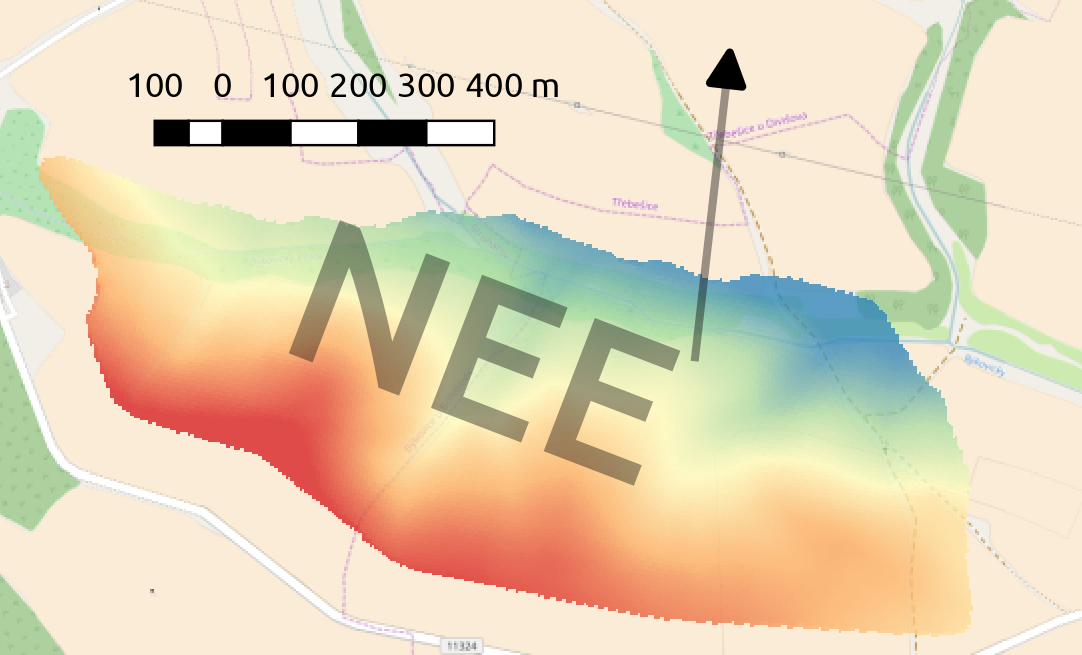
\includegraphics[width=0.5\textwidth]{./img/dmtbk.png}
  \caption{digitálního modelu terénu povodí Býkovice}
  \label{fig:bykovicedmt}
\end{figure}

\paragraph{Shapefile půd} \label{sec:vstuppuda}


V České republice se standardně používá na zemědělské půdě rozdělení půd podle zrnitosti dle Novákovi klasifikace . Půda je rozdělena podle obsahu tzv. jílových částic na půdy \cite{kavka}:
\begin{itemize} \itemsep 0pt
  \item písčité
  \item hlinitopísčité
  \item písčitohlinité
  \item hlinité
  \item jílovitohlinité
  \item jílovité
  \item jíl
\end{itemize}

Na lesních půdách je naopak využíván popis kategorií podle klasifikace USDA.
Vstupní shapefile popisuje prostorové rozložení jedotlivých půdních typů na řešeném území. Pro určení charakteristik je nutné aby obsahoval atributové pole udávající identifikátor daného půdního typu. Identifikátor odkazuje na půdní charakteristiky, které jsou definované v dalších vstupech (popsáno níže). Shapefile popisující půdu je zobrazen na obrázku \ref{fig:bykovicepuda}.
\begin{figure}
  \centering
  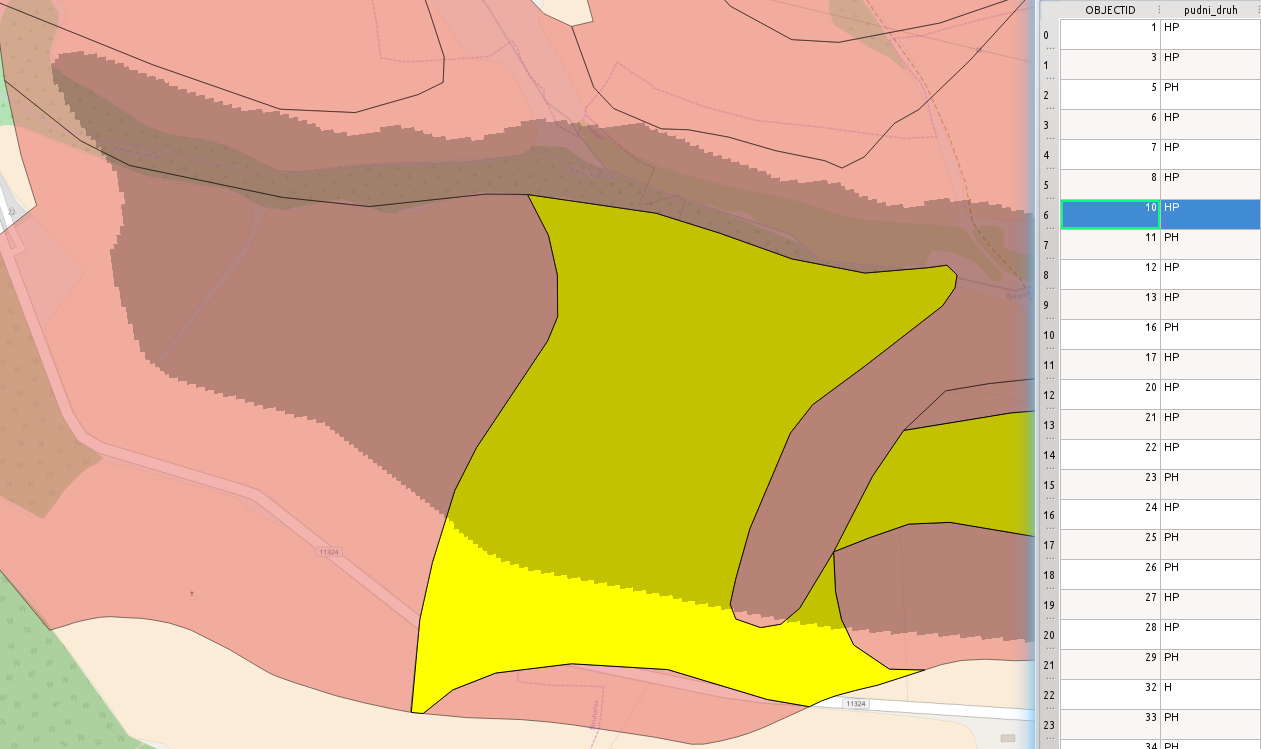
\includegraphics[width=0.5\textwidth]{./img/pudnityp.png}
  \caption{Ukázka vektorové vrstvy, atributové tabulky a polem v atributové tabulce (pudni\_druh) s identifikátorem půdního typu na vyznačeném území (HP).}
  \label{fig:bykovicepuda}
\end{figure}



\paragraph{Shapefile využití území} \label{sec:vstupvegetace}

Obdobně jako u půdních dat je vstupem vektorový shapefile popisující využití území. Mezi základní typy pro které byl model testován patří:
\begin{itemize} \itemsep 0pt
  \item atropogení a zpevněné plochy  
  \item holá půda bez vegetace
  \item les
  \item sad
  \item travní porosty
  \item zemědělské plodiny širokořádkové
  \item zemědělské plodiny úzkořádkové
\end{itemize}

\textit{Širokořádkové plodiny jsou například brambory, kukuřice, řepa, sója a slunečnice. Úzkořádkové plodiny jsou obiloviny nebo řepka.}
Shapefile popisující vegetaci je zobrazen na obrázku \ref{fig:bykovicevegetace}. Obdobně jako u půd v předchozí sekci je třeba atributovou tabulku tohoto shapefilu doplnit o identifikátor daného typu vegetace. Tento identifikátor odkazuje na charakteristiky daného vegetačního povrchu definované v dalším vstupech (popsáno níže).
\begin{figure}
  \centering
  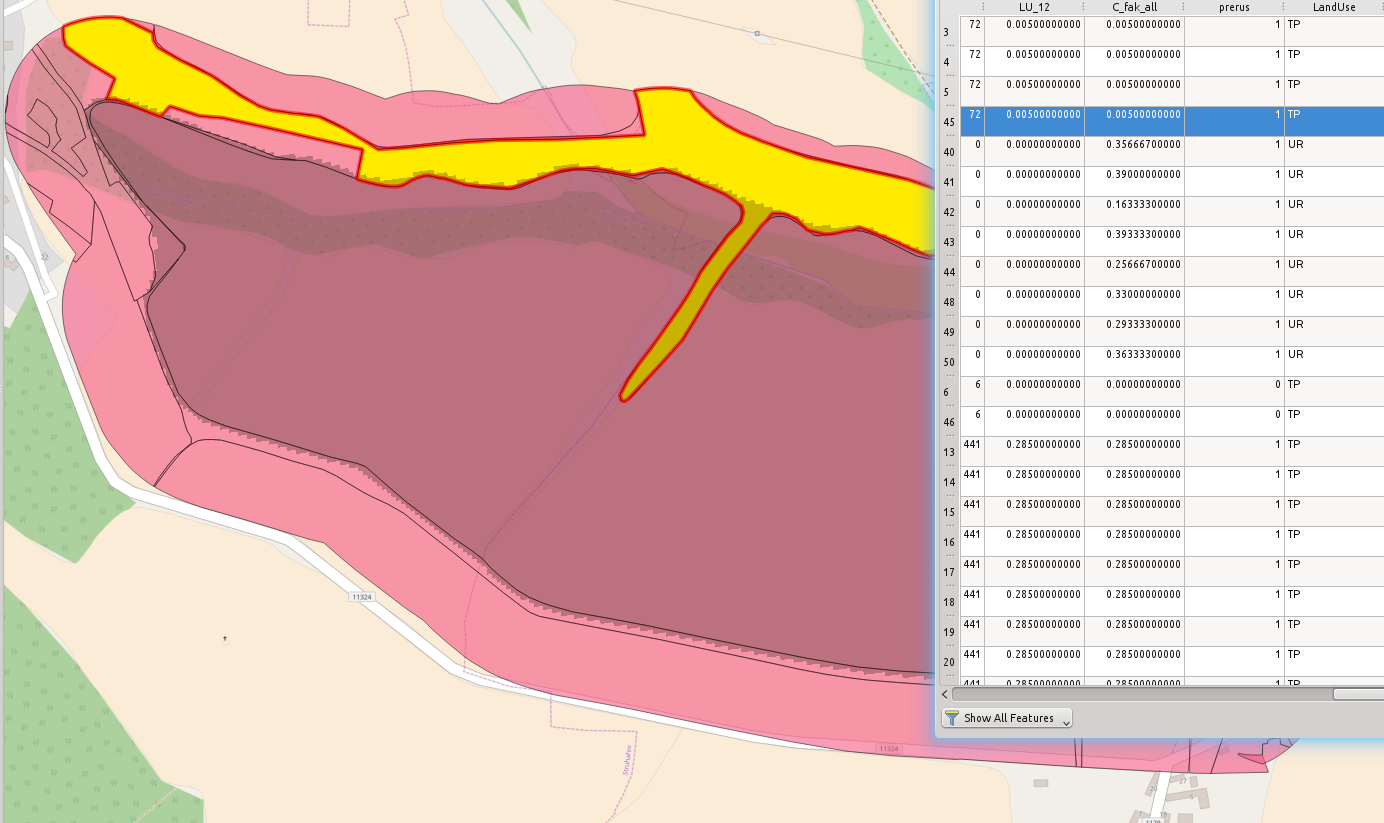
\includegraphics[width=0.5\textwidth]{./img/lu.png}
  \caption{Ukázka vektorové vrstvy, atributové tabulky a polem v atributové tabulce (LandUse) s~identifikátorem typu vegetace na vyznačeném území (TP - travní porost).}
  \label{fig:bykovicevegetace}
\end{figure}


\paragraph{Srážkový soubor} \label{sec:vstupsrazka}

Dalším vstupem je textový soubor obsahující srážková data. 
% 
% Na obrázku níže je ukázka textového souboru obsahující proměnlivou srážku, konkrétně je to měření na~rastru Býkovic ze~dne 8.2.2010.
%\begin{figure}[hbt]
%  \centering
 % \includegraphics[scale=1]{obrazky/srazkovysoubor.png}
  %\caption{Srážkový soubor}
%  \label{fig:srazkovysoubor}
%\end{figure}
% 
% 
Srážky se zadávají jako textový soubor se dvěma sloupci. V levém je časový interval v minutách v pravém \textbf{kumulativní úhrn} za daný časový interval v \textbf{milimetrech}. Například hodnoty na obrázku \ref{fig:srazkovysoubor} ukazují, že za prvních 10 minut běhu modelu naprší  na každou buňku rastru 3 mm, v období 10 - 60 minut 40 mm a od 60. minuty je srážka 0 mm. 
\begin{figure}
  \centering
  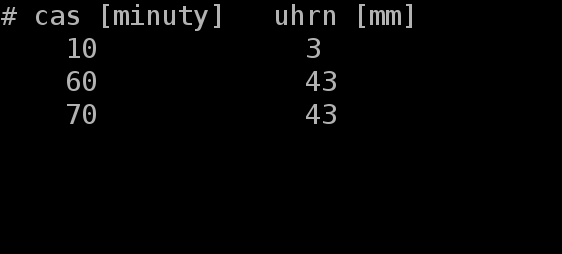
\includegraphics[width=0.5\textwidth]{./img/srazka.png}
  \caption{Ukázka srážkových dat. V intervalu 0 - 10 minut je úhrn 3 mm, v intervalu 10 - 60 minut je úhrn 40 mm a v intervalu 60 - 70 úhrn 0 mm}
  \label{fig:srazkovysoubor}
\end{figure}


\paragraph{Časový krok modelu (s) a celková doba simualce(min} \label{sec:vstupkrok}

Časový krok modelu označený jako \acs{dT} je hodnota v minutách, která udává velikost počátečního časového kroku. tento zadaný kro je maximální hodnout. během výpočtu je časový krok dynamicky zkracován podle Courantovy podmínky.. Velikost časového kroku tedy závisí na rychlosti děje a na velikosti prostorového kroku (velikosti buňky DMT). %Vzhledem k tomu, že rychlost odtoku v rýhám může být řádově vyšší než rychlost plošného odtoku je snaha řídit velikost časového kroku podle rychlosti plošného odtoku, kde Courantovo kritérium povoluje vyšší časový krok. Velikosti časového kroku zásadně ovlivňuje celkovou délku výpočtu. Pokud časový krok vyhovuje Courantovu kritériu v plošném odtoku, ale toku v rýhách již nikoli, začne se časový krok dělit pouze interně při výpočtu rýh. Tyto děje se probíhají při běhu programu a uživatel je nijak neovlivňuje, nicméně, je třeba si uvědomit, že při vytvoření rýhového odtoku a nutností dělit časový krok v těchto buňkách může se doba výpočtu jednoho časového kroku prodloužit. která udává velikost jednoho kroku výpočtu, v němž probíhá výpočet odtoku a další nedílné součásti programu. Zadaný časový krok se mění podle potřeb Courantova kritéria \ref{section:cfl}, nikdy však nemůže být vyšší než vstupní zadaná hodnota uživatelem. 

%Při zadávání počátečního časového kroku je možno zvolit hodnotu v rozmezí od 0.05 do 0.3 minuty. 
% Velikost časového kroku nejvíce ovlivňuje reálnou dobu běhu modelu. Čím nižší je časový krok, tím déle uživatel čeká na výsledky. 
%Stejně jako u všech ostatních číselných hodnot zadávaných do programu ArcGIS je potřeba myslet na to, že čísla s desetinnými místy musí být odděleny tečkou, nikoliv čárkou.
Délka běhu modelu je hodnota v minutách určující čas, do kterého se model po jednotlivých časových krocích dostane a skončí. Doporučená volba délky běhu modelu by měla být delší než zadávaná srážka.
 


%\paragraph{Povrchová retence} \label{sec:vstupretence}

%Povrchová retence je děj, při kterém se zachytává počáteční část srážky, která se dále neúčastní odtoku. V reálném prostředí si lze toto představit jako zachytávání srážkové vody v nerovnostech na povrchu. Pouze po naplnění těchto malých nerovností dochází k povrchovému odtoku. Hodnota závisí na hustotě půdy a její deformaci. Povrchová retence se zadává v mm. Pro veškerá testování byla povrchová retence zvolena 0.2 mm.

\paragraph{shapefile bodů pro generování hydrogramů} \label{sec:vstupbody}

Jedná  se o bodovou vrstvu. V těchto bodech se budou uživateli ukládat časové řady počítaných veličin. Tento volitelný vstupní parametr je podrobněji popsán ve výstupech \ref{sec:hydrogramy}.

\paragraph{Výstupní adresář} \label{sec:vstupadresar}
Výstupní adresář je složka, do které se uloží veškeré výsledné rastry a výstupní textové soubory. Na začátku běhu programu se obsah tohoto adresář celý vymaže, proto se doporučuje vždy provést kontrolu. V žádném případě nenastavujete jako výstupní adresář pracovní plochu, či jiný adresář, kde byste mohli mít uložena důležitá data!

\paragraph{Rýhový odtok} \label{sec:vstupryhovy}

Tento volitelný parametr po zaškrnutí umožní výpočet soustředěného odtoku. Soustředěný odtok je popsán v sekci \ref{sec:soustredenyodtok}.

\paragraph{Vícesměrný odtok} \label{sec:vstupvicesmerny}

Parametr volby vícesměrného odtoku je volitelný. Více o tomto typu odtoku je v části \ref{subsection:MD}

\paragraph{Tabulka parametrů půdy a vegetace}  \label{sec:upravatabulkyparametru}

Tento vstup je tabulka, na kterou se odkazují identifikátory půdního typu a typu vegetačního pokryvu v atributových tabulkách polygonových vrstev s prostorovým rozložením půd a vegetace. Tato tabulka může být do modelu vlože jako textový soubor. Na obrázku~\ref{fig:tabsoilveg} je ukázán příklad takové tabulky. V prvním sloupci jsou složené identifikátory (id) typu půd a typu vegetace. Na prvním řádku je ukázka odpovídající id půdního typu z obrázku~\ref{fig:bykovicepuda} HP a id typu využití území z obrázku~\ref{fig:bykovicevegetace} TP, které jsou v tabulce na obrázku~\ref{fig:tabsoilveg} spojeny na HPTP. Tímto způsobem je program schopen propojit prostorové uspořádání pud a typu vegetace s příslušnými charakteristikami. Spojení identifikátorů z atributových tabulkách polygonových vrstev prování program automaticky. Uživatel musí pouze zaručit aby se identifikátory v nastavené v atributových tabulkách polygonových vrstev schodovali s identifikátory v tabulce půdních charakteristik a charakteristik vegetace. 

Hlavničky druhého až posledního sloupce jsou povinné. Jejich význam je popsán v tabulce~\ref{tab:soilveg}. Názvy v druhém až posledním sloupečku musí být zadány malými písmeny.
\begin{figure}
  \centering
  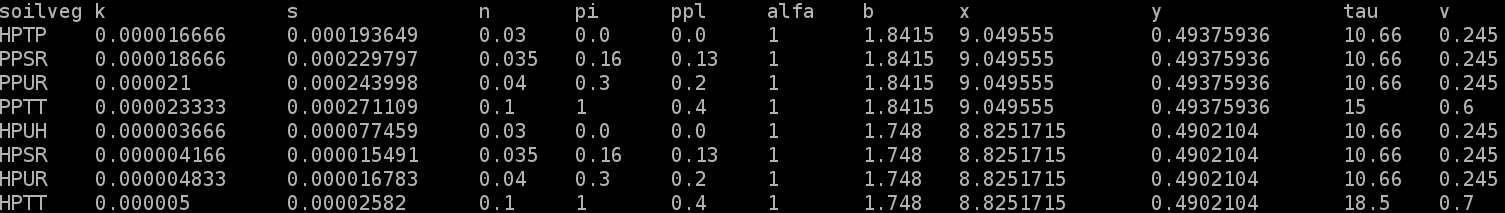
\includegraphics[width=1.0\textwidth]{./img/tabsoilveg.png}
  \caption{Ukázka tabulky s charakteristikami půd a vegetace. Význam veličin v jednotlivých sloupcích je popsán v tabulce~\ref{tab:soilveg}.}
  \label{fig:tabsoilveg}
\end{figure}

\begin{table}%[!htp]
  \centering
  \caption{Přehled parametrů charakterizujících půdní typ a typ vegetačního pokryvu}
  {\small
    \begin{tabular}{p{1.5cm}lp{4cm}}
    \hline
    Hlavička v tabulce & Symbol & Popis \\
    \hline \hline
    k&\acs{HyVod}  & \acl{HyVod} \\
    s&\acs{Sorb}   & \acl{Sorb} \\
    n&\acs{n}      & \acl{n}\\
    pi&\acs{PotI}   & \acl{PotI}\\
    ppl&\acs{Lai}    & \acl{Lai} \\
    ret&\acs{ret}    & \acl{ret} \\
    b&\acs{b}      & \acl{b} \\
    x&\acs{X}      & \acl{X} \\
    y&\acs{Y}      & \acl{Y} \\
    tau&\acs{taucrit}& \acl{taucrit} \\
    v&\acs{vcrit}  & \acl{vcrit} \\
    \hline
    \end{tabular}%
  }
  \label{tab:soilveg}%
\end{table}%

Meze jednotlivých parametrů jsou podrobněji popsány v kapitole XXX. 
Součástí manuálu jsou i vzorové tabulky.

\paragraph{Hydrografická síť} \label{sec:vodnitoky}

Hydrografickou sítí jsou myšleny nejen vodní toky, ale do modelu je možné zadávat i prvky dočasné hydrografické sítě jako jsou příkopy, průlehy, cesty s příkopy atp. Výpočet v modelu probíhá po zvoleých úsecích pomocí Manningovi rovnice pro výpočet průtoku. Prostorové úmístění jednotlivých prvků je formou shapefile (\textbf{Vrstva toků - Stream feature}). Jednotlivé vektory reprezentují úsek se stejnými charakteristikami. Tvar úseku, drsnost, základní průtok jsou pak zadávány pomocí externí tabulky kde jsou uvedeny charakteristiky pro jednotlivé typy úseků (\textbf{Tabulka vodních toků - Stream table}). Pro propojení prostorové informace s charakteristikami úseků je třeba mít v attributové tabulce shodný kód jako ve vrstvě vodních toků (\textbf{Kód vodních toků - Steam table code}).